\label{StateoftheArt}
I will define \acrfull{vr} and show the main characteristics of it through this chapter. Followed by listing several related projects that has been made in different places to immerse and show the user locations in different times. The last section will represent example projects that has been done in \acrshort{vr} in different places in the world focused on immigration, refugees and time traveling.   

\section{Virtual Reality}
Ivan Sutherland published a paper entitled "the ultimate display" in 1965 describing how computers would one day open a window to the virtual world for the user. He created a \acrfull{hmd} in 1968, it is a display device that is worn on the head and had a display for each eye, which displayed left and right views of a computer-generated 3D scene to the user so that the digital scene remained static when the user's head was shifted. The images, as they were simple line drawings, were far from reality. But as they were stereoscopic, the user had the impression of looking at a solid 3D object, Which is now seen as the birth of Virtual Reality \citep{Vince2011}.  

Virtual Reality is a technology that is often regarded as a natural extension of 3D computer graphics with specialized input and output tools \citep{Jayaram1997}. Ryan (2001) defined it as an “interactive, immersive experience generated by a computer” \citep{Ryan2001}. And according to G.C. Burdea and Coiffet (2017) “it is a generated computer graphics used to create a realistic-looking world that responds to the user’s input (gestures, verbal commands, etc.)” \cite[p.20]{burdea2017virtual}. Instead of seeing a screen in front of them, the users will be engulfed in a 3D environment by virtual reality.“The scientific community has been working in the field of virtual reality (VR) for decades, having recognized it as a very powerful human-computer interface”\cite[p.19]{burdea2017virtual}. 

As shown in Figure \ref{fig:3I} In order to build a reliable virtual environment, three elements are needed:  immersion, interaction, and imagination. They are called the “3I’s” of virtual reality \citep{Hu2016,burdea2017virtual,Bamodu2013VirtualComponents}.

\begin{wrapfigure}{r}{0.30\textwidth} %this figure will be at the right
    \centering
    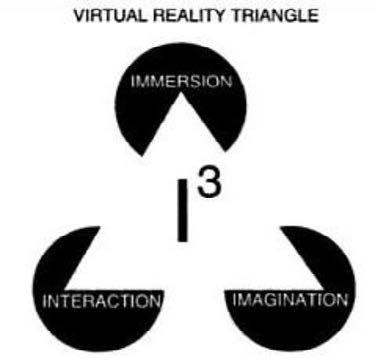
\includegraphics[width=0.28\textwidth]{3I}
    \caption{The 3I's of Virtual Reality - © 2003 by John Wiley \& Sons Inc. All rights
reserved}
    \label{fig:3I}
\end{wrapfigure}



1. \textbf{Immersion:} It is the situation of virtual reality in which the user feels inside the scene personally and immerses himself in the simulated virtual world.



2. \textbf{Interaction:} The user-to-virtual environment interactive feedback. Since it is an interface between man and machine, the system should immediately respond to the actions of the user.




3. \textbf{Imagination:} For a better user simulated experience, the scene structure and the construction of the environment were formulated with imagination.

\section{Types of Virtual Reality Systems} \acrshort{vr} technologies have been categorized into three main categories, Non-immersive system, semi-immersive system, and Immersive system, according to \cite{Bamodu2013VirtualComponents}. This is based on the system's level of immersion, interface, and components used.  

\textbf{Non-Immersive VR system}
It is also called the World system's desktop \acrshort{vr} system, Fishtank or Window is the least immersive and least expensive of the \acrshort{vr} systems because it needs the least complex components. This uses traditional graphics workstations with a screen, a keyboard, and a mouse, with modeling and \acrfull{cad} systems in its software areas.  

\textbf{Semi-Immersive VR system}
Use a relatively high-performance graphics computing system coupled with a large surface to display the visual scene, provide high immersion levels while maintaining desktop \acrshort{vr} simplicity or using some physical model. One such program is the \acrfull{cave} also, the driving simulator as a semi-immersive system \citep{Bamodu2013VirtualComponents}. 

\textbf{Immersive VR system}
 The immersive \acrshort{vr} system is the most expensive and provides the highest level of immersion, its components include \acrfull{hmd}, tracking devices, data gloves, and others that include the user with computer-generated 3D animation that gives the user a sense of being part of the virtual environment. \citep{Bamodu2013VirtualComponents, Baus2014MovingReview}.

\begin{figure}[ht]
    \centering
    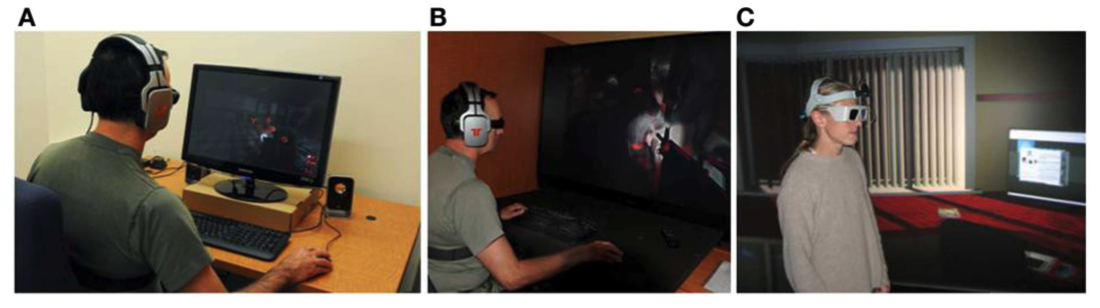
\includegraphics[width=0.98\textwidth]{images/vrsystem.png}
    \caption{VR Systems A: non-immersive system, B: semi-immersive system, C: Immersive system \citep{Baus2014MovingReview}}
    \label{fig:vrsys}
\end{figure}


\section{Presence in Virtual Reality} 
Due to powerful simulated influence, the user will experience emotional and physical response as if the virtual world happened physically \citep{Waterworth2014}. The sensation of being in a real place, as well as the perception of validity, getting the sense that the scenario is taking place. Although the user knows that the virtual world is just a simulation, these illusions occur. \acrshort{vr} has been one of the main trends in the evolution of presence \citep{Waterworth2014, Steinicke2016}. In
\acrlong{vr} the interaction ranges from purely visual interaction to differentiated contact that the user can communicate with objects in virtual reality with the perceptions and cognitive processing capacities experienced in the real world, and the sensation is similar to the changes in the natural world \citep{Hu2016}.
\acrshort{vr} gives the user the ability to control, move and look in the virtual world, which has a significant impact on the level of presence, hence the greater the user's sense of immersion \citep{William}. \say{When we feel a strong mediated presence, we react emotionally and
bodily (at least to some extent) as if the virtual world existed physically}\cite[p.4]{Waterworth2014}.


We need to understand the \acrfull{fov} and the \acrfull{for} for a human to achieve a significant level of immersion for the user. The human \acrshort{fov} is about 200 degrees with a binocular overlap of 120 degrees. The field of view of the display is a measure of the angular width of the vision of a user that is covered at any time by the display as shown in Figure \ref{fig:field}. Due to the edge of the screen, the field of view is reduced in a three-sided \acrshort{vr} projection, but it is 100\% if the user looks forward to it. Nevertheless, throughout the three-sided stationary projection, the stereo range is broader, several \acrlong{hmd}'s provide a 100-120 degrees of \acrshort{fov} which is a sensible part of the human visual range for providing a high resolution footage. Even though the stereo overlap is very essential and can differ in \acrshort{hmd}'s where the two displays are more or less broadly separated, it will be difficult to perceive stereopsis if the overlap between the two eyes is as small as 30 degrees \citep{William}.
If the user moves towards an object, the ciliary muscles adjust the lens shape to handle the emitted light waves to keep a picture in focus. The eyes also intersect automatically to ensure that the refracted images fall on the two retinas similar areas. The cause of stereoscopic vision is this method of projecting an object to specific locations on the two retinas. The discrepancy between the retinal images is termed binocular disparity and is used to measure distance, resulting in a three-dimensional context \citep{Vince2011}.

\begin{figure}[ht]
    \centering
    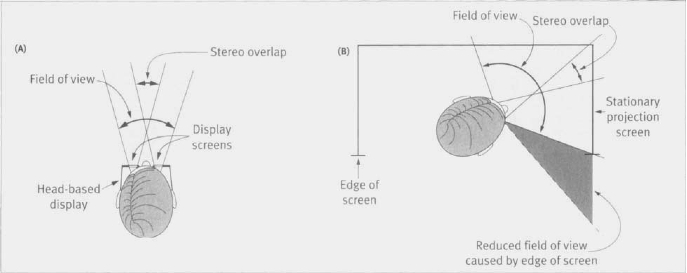
\includegraphics[width=0.80\textwidth]{Fod.png}
    \caption{Field of View - \citep{William}}
    \label{fig:field}
\end{figure}


\begin{figure}[ht]
    \centering
    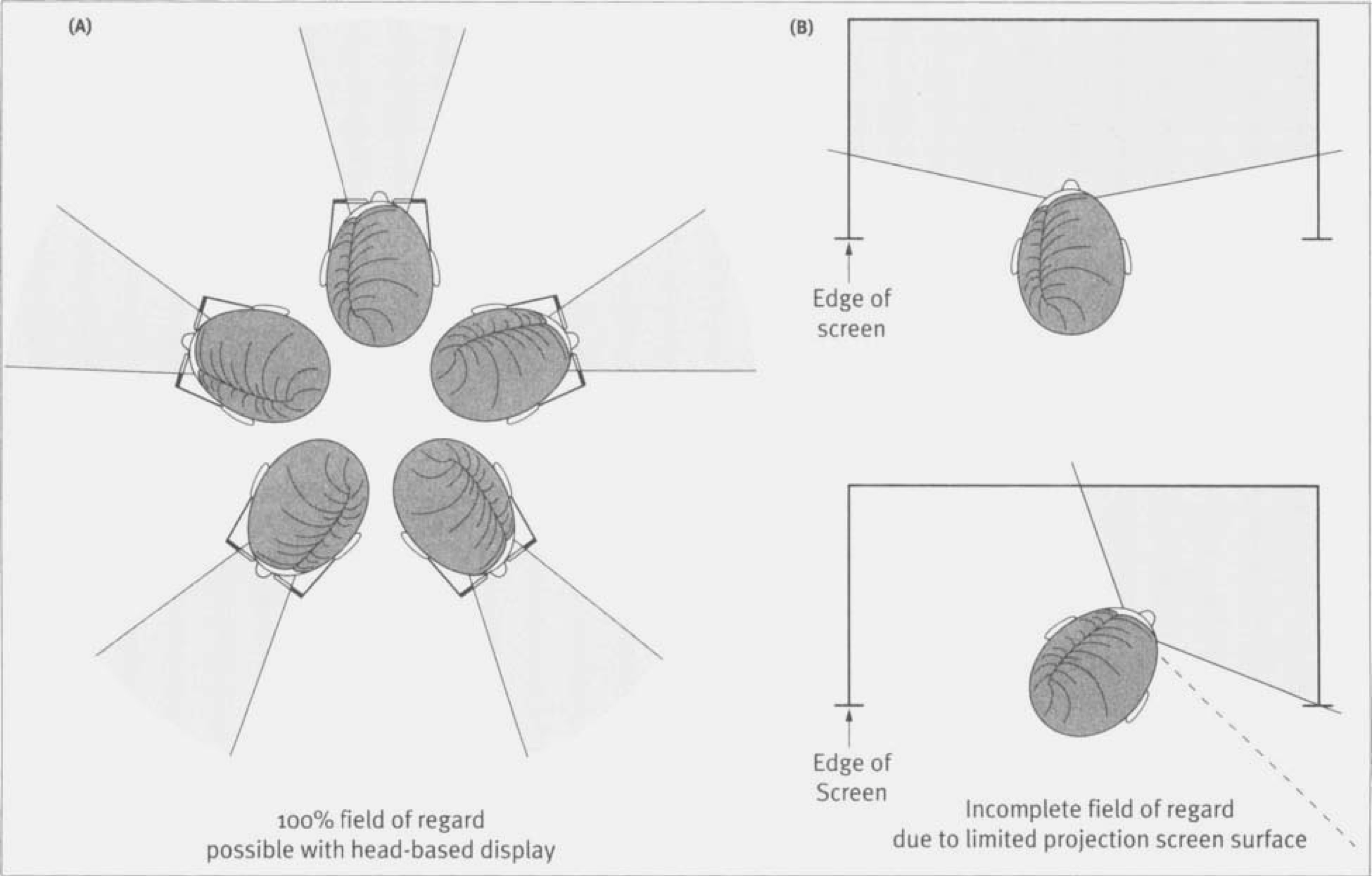
\includegraphics[width=0.90\textwidth]{fov.png}
    \caption{Field of Range - \citep{William}}
    \label{fig:fod}
\end{figure}

The \acrfull{for} is the amount of space within the virtual world that surrounds the user. As shown in Figure \ref{fig:fod}, due to the displays that always face the user's eyes, the \acrshort{for} in the \acrshort{hmd} is 100 percent, regardless of the direction that the user stares at, the virtual reality would always be in front of his eyes. In the three-sided \acrshort{vr} projection, the \acrshort{for} is usually less than 100 percent because the virtual environment will always need projectors and it will not be dynamic in motion as the \acrlong{hmd} \citep{William}.

A \acrlong{hmd} is nothing but a stereoscope, which uses not just pictures but animated video clips as well. What is significant, however, is that the images seen by both eyes must overlap and stereoscopic vision is experienced in this field of overlap \citep{Vince2011}.
This stereo-overlap zone is shown in Figure \ref{fig:field}. Since the two images are captured from two different visual locations, the brain uses these variations to create a single image containing information about distance \citep{Vince2011}. Thus, the use of \acrshort{hmd}'s could have its repercussions, e.g. a low latency monitoring "not more than 2ms (millisecond)" is needed to adjust the screen picture to the viewer's physical movement also to prevent movement discomfort because high latencies have serious negative consequences on simulation, e.g. vomiting, nausea or vertigo \citep{burdea2017virtual, Vince2011, Steinicke2016}.

Smartphones have created a technological revolution, merging communication and computing devices, where they are small in scale and can fit into the pocket of the user. The high computing power permitted in smartphones is adequate to handle the \acrshort{vr} world, Google and Samsung have launched primarily smartphone-based \acrshort{vr} headsets like Google Cardboard and Samsung's Gear VR, where the user can place the smartphone within the headset, and experience Virtual Reality, Subsequently, the smartphone will provide a split display for the headset lenses. Thereby allowing a lightweight and realistic \acrshort{vr} interface and web renaissance of \acrshort{vr}. The main elements of smartphones today, such as high-density display panels, gyroscopes, and accelerometers, are installed in most models and therefore cost only a fraction of the Virtual reality system value in the early 1990s \citep{Steinicke2016}. 



  
\section{Benefits of Virtual Reality}

Virtual reality is a technology that offers users with multiple benefits and displays successful results in various aspects. Virtual reality is also useful for simulating inherently dangerous activities (e.g. coal mining) by providing an immersive real-life training scenarios for the workers to manage different types of hazards \citep{VanWyk2009VirtualIndustry}. Also, training users on expensive equipment (e.g. aircraft) tasks. Without compromising their safety, users can perform hazardous tasks by executing training on the duties via Virtual Reality before applying it in reality. With a risk-free environment, virtual reality allows users to make and take decisions \citep{Aguinas2004}. While it is a risk-free environment, such as surgical practice, it has enabled its experiences by researchers in education. Traditionally, medical education apprenticeship has been done under the guidance of a professional physician while the surgical trainee trains to perform surgery. Virtual reality learning reduced the time required to complete a mission, improved accuracy, and reduced errors \citep{Ks2009}. Virtual reality captures the curiosity of the student. They find engaging and walking through a virtual environment exciting and challenging. Students can study in-depth and make new findings. Also, people living with disabilities can engage in an atmosphere of exploration and training. We can do tests in chemistry and physics and practice how to do them \citep{Pantelidis2010}. Virtual rehabilitation described as treatment delivery using the hardware and simulations of Virtual Reality. It is helpful for people with post-traumatic stress disorder (PTSD) or patients who are afraid of flying or other fears. According to 
\cite{Burdea2003} 92 percent of people who were afraid to fly maintained their success and flew on flights \citep{Burdea2003}.

Virtual reality has a positive effect on social and psychological directions, for instance, it can reduce anxiety for people who have the fear of public speaking. \cite{Chang2019StereotypeOutcomes} discussed how women achieved higher scores in math when they studied math over a virtual environment and they used male avatars in \acrshort{vr}. Therefore, avatars can affect interpersonal dynamics by incarnating a minority race, therefore it would decrease the bias against the minorities \citep{Markowitz2018ImmersiveChange, Chang2019StereotypeOutcomes}.   

 A color-blind experiment was conducted to test the user's supporting behavior. By arbitrarily checking the colorblind perception of Virtual Reality for some participants, and others just imagining that they had red-green blindness. After that, participants were asked to assist color-blind people. Those who have experienced color-blindness in Virtual Reality were more willing to help than the ones who imagined the color-blindness. It means that the embodiment of virtual reality is more powerful than the imagination of the mind \citep{Shriram2017VirtualBehavior}. VR presents us with the ability to go further than these physical limitations. Within VR, individuals can break laws of physics to alter their appearance, skills, and atmosphere. Immersive virtual reality technology makes it possible to \say{change the nature of social interaction}. Users can distinguish their actual behavior and appearance from their simulated representations, contributing to behavioral and social implications for both the digital and physical world \citep{Shriram2017VirtualBehavior}.
Several projects will present the role of virtual reality in accomplishing new experiences and enhancements in some fields.

\textbf{The Machine to be Another} \footnote{The Machine to be Another - \url{www.beanotherlab.org}} : A system of virtual reality that enables people to experience the world through the eyes and body of another person. Cognitive science, performance, and virtual reality make it possible for users to see themselves in a different body while interacting with the surrounding space and receiving realistic feedback. Based on long-term studies on how compassion can be encouraged in resolving issues such as cultural bias, diversity, conflict resolution, and body extension among others. The system also functions as a consequence of narrative, also a very useful framework in psychology and health care.
The system is designed for an open community of creators, scientists, and individuals with a common dream of building an empathic society. The BeAnotherLab's purpose is to encourage human integration through technical and scientific knowledge.

\textbf{Chernobyl VR} \footnote{Chernobyl VR - \url{www.chernobylvrproject.com}} : Chernobyl VR Project is made by The Farm 51,  it is integrating video game with an application for instructional and storytelling film. It is the very first virtual tour around the Chernobyl and Pripyat area. The project has been designed with state of the art technologies like 3D scans of locations and buildings, spherical photography, stereoscopic videos. 


\textbf{IrisVR} \footnote{IrisVR - \url{www.irisvr.com}} : A VR platform that enables engineers and customers to experience the designs in a space of real scale. IrisVR captures and transforms every 3D file into a walkable VR world. Iris is compatible with multiple Head-mounted displays, therefore the users can have meetings inside the space since Iris supports a multi-user experience provided with a reliable voice chat and a shared virtual environment for presentations and design reviews.


\textbf{AVR EON reality} \footnote{Eon Reality - \url{www.eonreality.com}} : EON Reality created eight AVR training modules for NTU students and staff in the chemistry laboratory. Using a head-mounted display in virtual reality, students and staff can improve their awareness and manage different disaster situations remotely without any of the potential hazards or costs. EON Reality's Virtual Trainer solution provided risk-free safety and prevention training for some of the most common chemical laboratory emergencies, from preventing and controlling chemical hazards to protecting the health and safety of colleagues within the laboratory.

\section{Storytelling in Virtual Reality}

Virtual reality technologies are rarely implicated in fundamental social or cultural activities. The development of immersive environments in virtual reality is a significant socio-technical issue. If the user does not experience enough immersion it would be difficult to get the user to believe the scenario in the \acrshort{vr} setting \citep{Darcy2003VirtualStorytelling, Steinicke2016}. It would be helpful to merge \acrlong{vr} with interactive storytelling and to make enhancements in practical training. Among storytelling and training, there is a strong synergy. Immersive \acrshort{vr} can therefore improve and increase the confidence and curiosity of the trainee about transferred knowledge and retention \citep{Ponder2003ImmersiveTraining}. Storytelling in Virtual reality is an intensive research topic, even though there are no clear guidelines for 360$^{\circ}$ storytelling \citep{Gugenheimer2016SwiVRChair:Reality, Ponder2003ImmersiveTraining}. Many people tried different experiments to bring new technology to the traditional narrative but most of them have failed \citep{Balet2003VirtualProceedings}. Disney as a pioneer in storytelling published a paper in 1996 for their first steps of storytelling in virtual reality after applying it to an installation where guests travel through the virtual world of a magic carpet based on the original Disney movie “Aladdin” \citep{Pausch1996DisneysReality}. Disney came up with some conclusions, a) Content matters: even with high fidelity Virtual reality is not enough, because the user focuses on what there is to do in the environment. b) Users need a background story: to get the user familiar with the new environment he needs to get provided with a background story before the immersion. c) Users need a goal: where the user needs to know what is the purpose to be in a virtual world. d) Tell a straightforward story: when the user is perceptually overwhelmed it helps to keep the story short and clear \citep{Pausch1996DisneysReality}. However, we can not compare games with stories,\say{we typically enjoy stories passively, and usually as individuals even while sitting in a group audience} \cite [p.52]{Balet2003VirtualProceedings}. In other words, we enjoy the story of Luke Skywalker in Star Wars films, but when we became a Jedi Knight in the Jedi Knight game it would be less impressive hence the user gets the potential to find and tell his own story not the author \citep{Balet2003VirtualProceedings}. However, the narrative is adaptable almost in any communication medium, but it needs to be characterized for the medium, \citep{Balet2003VirtualProceedings} listed characterization for considering virtual storytelling:
\begin{itemize}
\item Levels of Meaning like the level of action, also the linear development of narrative structure.
\item A confusion of consequence i.e. what is caused by what.
\item The narrative will always seek to prolong its life. 
\item Time is relative to the narrative logic. 
\end{itemize}
Narrative is really important factor in virtual reality specially for immersion, it needs to be structured regarding to the scenes and the design of the virtual environment.  

\section{Example Projects}




\textbf{Auschwitz Virtual Tour}\footnote{Auschwitz VR Tour - \url{www.youtube.com/watch?v=EOM_CxAKB_Y}}:
The German broadcasting institution WDR made a 360$^{\circ}$ documentary in Auschwitz concentration camp. Within the documentary, some Holocaust survivors tell their stories. While listening to the stories and seeing the different locations in the camp the user could feel the fear and horror that people suffered from. The video immerses the user through the sound of the surrounding environment in the camp, you can hear the wind and the sound gives a slight feeling of the cold weather over there. The experience is immersive, but there is no interactivity with the user.





\textbf{Clouds over Sidra}\footnote{The Za’atari camp VR Tour - \url{www.youtube.com/watch?v=mUosdCQsMkM}}: 
12 years old girls’ daily life story at the Za’atari refugee camp in Jordan
showed in virtual reality. The camp is a home for 80,000 Syrian refugees, half of them are children(“Syrian Refugee Crisis – UN Virtual Reality,” 2015). The documentary was made by the United Nation to raise awareness about the Syrian crisis. The video contained a number of short videos from different parts of the camp, and it’s being synchronized while Sidra narrates her story.
It is more like watching a video with empathy than being immersed, but
the video presents the real life of the camp. Although the difference that while watching and
listening to the story, the user observes the people how they actually survive and live in the
camp. Therefore, the user does not have to imagine how is life over there.



\textbf{Carne y arena}\footnote{Carne y Arena Trailer - \url{www.youtube.com/watch?v=zF-focK30WE}} : A highly professional
Virtual reality project that puts viewers
into the harsh life of an immigrant. The
user is placed among a group of
Mexican immigrants passing the
borders into the U.S. It was written and
directed by Alejandro G. Iñárritu. 
It Is a full virtual reality experience; the user
needs to reserve an individual session
on the website. According to Pinotti (2017) you go in a dark room; your feet are on the sand (coarse grain, rough feeling) then, two assistants welcome you and provide you with the
necessary devices: an Oculus Rift headset, a backpack connected via cables to a powerful
computer and you are ready to be caught up in a nightmare \citep{Pinotti2017}. The project is
subtitled by ‘Virtually present, Physically invisible’. 


Pinotti (2017) defined, Virtually present:
“you are transported in the middle of the desert, among men, women, and children who try
their voyage of hope”. Physically invisible: “you are present, but nobody sees you and after a
while, you start to feel the need to be noticed and seek acknowledgment of social
recognition” \citep{Pinotti2017}. 
\begin{wrapfigure}{R}{0.20\textwidth}
    \centering
    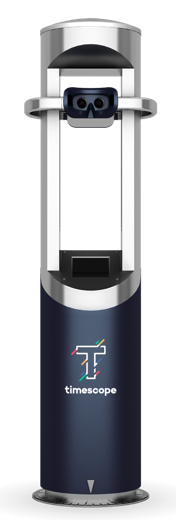
\includegraphics[width=0.16\textwidth]{timescope.png}
    \caption{Timescope terminal - © timescope.com }
    \label{fig:timescope}
\end{wrapfigure}
The project was developed with high technology, like 3D
modeling, visual effects, sound. The interaction of the user and the feeling of “being there”
by placing the user in a special environment, leads to a unique experience of immersion.

\textbf{Timescope}\footnote{Timescope - \url{www.timescope.com}} : A \acrshort{vr} terminal that installed in the street. It gives the user the ability to explore the location at a different time. The terminal first installed at the Place de la Bastille in Paris. Where nothing remained of that historic place since it was demolished in 1789. Timescope developed this \acrshort{vr} terminal as shown in Figure \ref{fig:timescope}. Thus, it gives people the ability to travel back in time and see the Bastille in 1416. Where it was first completed, or to 1789 where it was seized by revolutionaries. The 360 images and videos that are provided in the Timescope terminal gets the user immersed.

In different locations, the terminal also provides futuristic projects, to discover what would the location look like in the future \citep{Hiner2016HowTechRepublic}. 

\textbf{Palestine 360}\footnote{Palestine 360 - \url{www.360.ps}} : A platform based on WebVR technology. It shows 360 images from different sites and locations in Palestine. The website gives the user the ability to use VR glasses to experience 360 high-quality images. The images show not only historic locations but also restaurants and hotels. Some locations have background music and sometimes a narrator explaining the visited site. Some cities have a large-scale map on the right-side inside the VR experience. In a few scenes, there is a location-pointer where the user can use the gaze feature as a click to get transported to a new scene. 


\textbf{Palestine VR App}\footnote{Palestine VR - \url{www.pipd.ps/2019/10/28/download-palestine-vr}} : The Application shows videos of real-life in Palestine. Each city in Palestine is represented by a different person. The presenters are holding the 360 camera while they walk around the city or the location. The app included videos from different cities Jerusalem, Hebron, Gaza City, Bethlehem, Ramallah and Khan Al Ahmar. Videos need to get downloaded each time you use the application. thus, it might take some time to load the content on a slow internet connection. The Application has a different kind of a user interface when you activate the VR glasses mode. It has a gaze feature for selection, and the user can be transported between the scenes. Either by selecting the next scene by the bottom down video controllers or by getting back to the menu. 

\textbf{Time Ride}\footnote{Time Ride - \url{www.timeride.de}} : A guided tour that travels with the user in different old times in different locations around Germany. Timeride is a physical location for the public and tourists so they can see the city in a different scope of time. 
\begin{figure}[ht]
    \centering
    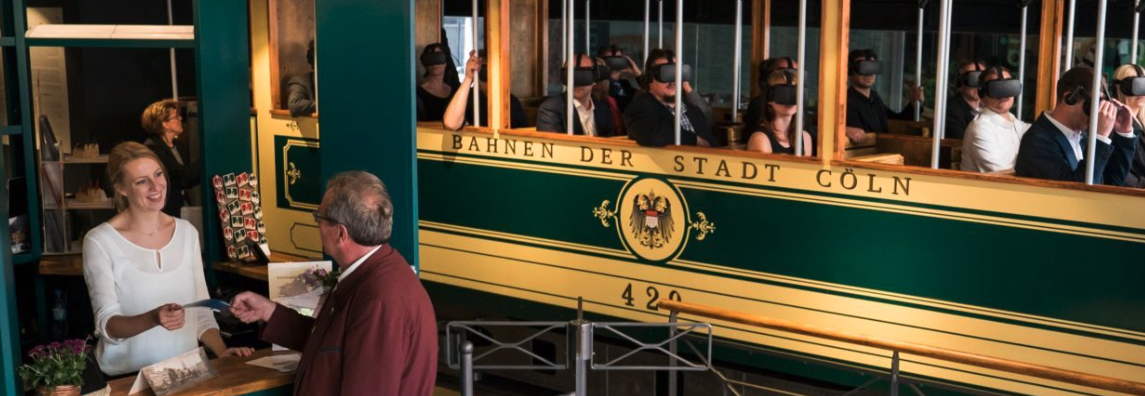
\includegraphics[width=0.98\textwidth]{images/timeride.png}
    \caption{Timeride in Cologne - © timeride.de }
    \label{fig:time}
\end{figure}
Timeride exists in Cologne, Dresden, Munich, and Berlin. In Cologne, the user will experience the imperial age of the city while sitting in a tram cabin as shown in Figure \ref{fig:time}. While in Dresden the user will travel back to the Baroque era in 1719. The user will witness Bavarian history in Munich while sitting in a peacock wagon. Also in Berlin, the user will enjoy a journey in the '80s.





\section{New Media in Conflict}

After the occupation of Palestine in 1948, a lot of Palestinians were expelled from their houses and villages and they became refugees in other countries, I will explain it in detail in the next chapter.  
There are many different locations in the world where the Palestinians are dispersed since they have no country of their own. The Palestinians used chat rooms and websites to share their daily life suffering stories, and the internet even revolutionized Palestinian relations in the diaspora and Palestine \citep{Ogunyemi2015, Aouragh2011}. Nevertheless,\say{It could help defy the repression of everyday life in Palestine by overcoming the limitations of checkpoints and occupation and thus generate feelings of ‘mobility’ and ‘political autonomy'}\cite [p.1]{Aouragh2011}.

Most Palestinian refugees want to return to Palestine, but they do not think they can, but the internet will allow physical borders to be avoided and boundaries to be resolved, Palestinians divided by national borders and roadblocks or by geographical and political obstacles have been able to show new ways of communicating by creative grassroots projects \citep{Aouragh2011}. 


According to \cite{Wulf2013} In the late 1990s, the Palestinians began telling their narrative to the world on the Internet as it led to a digital media activism \citep{Wulf2013}. Palestinians used emails and Facebook to organize protests and provide the outside world with more pictures and information to demonstrate the Palestinians daily suffering under Israeli occupation \citep{Wulf2013}. However, on digital media channels, the Israeli government followed the Palestinians, for instance, it requested from Facebook to drop the page \say{Third Palestinian Intifada} and from Apple to withdraw the \say{Third Palestinian Intifada} App from the App Store \citep{Wulf2013}. 

During the second intifada and before Facebook, the Palestinians used emails, websites, and blogs. Technological development has given the websites a broader context by providing multi-lingual content and a user-friendly interface. It increased the performance and availability which helped to expand the audience's reach \citep{Aouragh2011}. Today, Palestinian communications are more accessible, using Facebook WhatsApp, and other social media to communicate with the outside world. While 3G technology only arrived in Palestine in 2018 due to Israeli frequency restrictions. Communication in Palestine is necessary to understand because it's like a two-edged sword. Communicating with people is easier, but on the other hand, it is being monitored by Israel, particularly social media platforms.  Understanding the effect of communications on Palestinians and the influence of Palestinians on the media is therefore important.

\section{Research Gap}

I listed several platforms in the previous sections during the study and my exploration in various technologies and applications relevant to virtual reality entertainment, storytelling, and time travel. From a regional and technological context, I considered a research gap between all those platforms where it also implies on usability and user experience. Most of the time-travel projects are based in Europe, I haven't seen any time traveling platform in conflict countries. These time-travel platforms are stationary from a technical point of view, they are not easily accessible to everyone. The Paris Terminalscope is installed on the street sidewalk, but if you weren't in Paris and not directly in that sidewalk, you won't be able to see the Bastille in virtual reality. In Palestine it was different, to show different locations in Palestine, two \acrshort{vr} platforms were built. The first is a website that can be used by anyone, it has a feature that allows the user to view the place through the smartphone via a \acrshort{vr} headset. This Website offers only 360 pictures of Palestine's cities and places. In comparison, the photographs are empty they barely contain any human appearance, where that does not reflect the location's real-life. Technically, the mobile app doesn't have an interface, whenever the user wants to see another place they need to take the phone out and search for a new spot on the website. Nevertheless, the \acrshort{vr} experience is not reliable after trying it on different devices, it was not stable and the image was flicker's on some devices. The second application contained videos that are filmed while the narrator is holding the camera and tells the story of the place. The narrator's face is very close to the camera and that makes it uncomfortable for the user to see or listen to him. The second issue with this application is motion. Moving with the camera through different places that would cause motion sickness. Optic flow caused by moving visual imagery even if the \acrshort{vr} user is standing still would lead to motion sickness \citep{Steinicke2016}. 
Technology gave the ability for Palestinians to tell their story upon the world, further to have easier communication with Palestinians in the diaspora. There is no mobile application that provides the user with the ability to see real life in Palestine. Although there are VR mobile applications, they lack in immersion, interaction, and imagination. The narrative is a significant factor for immersion. The user should be able to travel back in time and see how some places looked like while listening to the narration. The Palestinians can show and tell their story in an immersive medium like Virtual Reality. The application would enrich the connection between the Palestinians in the diaspora and Palestine. It would let them experience life there without passing any borders.
 

